%% ------------------------------------------------------------------------- %%
\chapter{Study pipeline}
\label{cap:study-methodology}

The main objective of this work is to study and compare the impact of selected hyperparameters in different models trained on different datasets, using the LightGBM gradient boosting algorithm. Each "type" of dataset will be aggregated in different categories using the values of aggregated characteristics of the dataset itself (e.g. number of features, number of instances), this can be checked on section \ref{dataset-aggregated-statistics}.

In the following sections an overview about the methodology and experimental setup is given, explaining the datasets, the hyperparameters chosen and its distributions, pipeline for testing and the tools used in each step.

%% ------------------------------------------------------------------------- %%
\section{Tools}

All of the study pipeline and analysis is done using Python 3.6. Besides the commonly used data science tools (\textit{numpy, pandas, matplotlib, seaborn}) the most important packages used are:

\begin{itemize}
    \item \textbf{fklearn}: Functional machine learning library, developed by Nubank and built on top of \code{scikit-learn} and main machine learning implementations, e.g. the \code{LightGBM}; It has very useful abstractions, used in this study to build a pipeline of multiple learners and applying the same evaluation function;
    \item \textbf{toolz}: Add more functional programming functionality into python, trying to follow the principles of composability, purity and laziness.
    \item \textbf{scikit-learn}: The most widely used machine learning library for python;
    \item \textbf{pingouin}: Statistical package, mainly used for ANOVA tests and Levene's test for homoscedasticity. More details about it can be found in \cite{Vallat2018};
    \item \textbf{scipy}: Scientific computing package, the most used module was \code{scipy.stats} for statistical tests on the experiment results;
    \item \textbf{scikit-posthoc}: Library from the \textit{scikit} environment, which provides post hoc tests for pairwise multiple comparisons that are usually performed in statistical data analysis to assess the differences between group levels if a statistically significant result of ANOVA (or the equivalent nonparametric test) test has been obtained, more details in \cite{Terpilowski2019}.

\end{itemize}

%% ------------------------------------------------------------------------- %%
\section{OpenML Datasets}

The OpenML project has an online service to ``(...) share, organize
and reuse data, code and experiments. Following best practices observed in other sciences, OpenML allows collaborations to scale effortlessly and rewards scientists for sharing
their data more openly'' (\cite{Vanschoren:2014:ONS:2641190.2641198}).

In the research of previous studies for this work, it was noted that OpenML was being used in different scientific studies related to machine learning; A specific subset of datasets was used in \cite{probst2018tunability} to conduct a large-scale benchmarking to measure hyperparameter tunability, and it was also used in \cite{couronne2018random} as a benchmark platform for automatically retrieving datasets and comparing different machine learning algorithms.

OpenML provides a python API package for automatically retrieving datasets, tasks, submit customized runs and obtaining OpenML flows (a description of a personalized machine learning task). In this study, the datasets used are retrieved using the python API, and filtered according to some personalized rules, which are:

\begin{enumerate}
    \item  \textbf{\code{classes} = 2}, the study consists of analyzing binary classification problems;
    \item  \textbf{\code{min\_num\_features} = 3}, the dataset must have at least 3 features;
    \item  \textbf{\code{min\_num\_instances} = 1000}, the dataset must have at least $1000$ instances (data points);
    \item  \textbf{\code{max\_num\_instances} = 5000000}, the dataset must have at most $5$ million data points (provided just as an upper bound, no dataset used had more then $2$ million instances);
    \item  \textbf{\code{max\_nan\_percentage} = 20\%}, LightGBM has built-in support for missing values (\textit{NaNs}), but the datasets are filtered to have at most 20\% of its total number of rows with some missing values, for more meaningful data and simplicity.
\end{enumerate}

\begin{figure}[!h]
    \centering
    \includegraphics[width=1\textwidth]{openml_eda1.png} 
    \caption{Number of datasets after filtering is close to 400}
    \label{fig:openml-eda1}
\end{figure}

After all these filters, the number of valid datasets for the experiment would be close to 400 (figure \ref{fig:openml-eda1}), in theory. However, a lot of datasets could not be opened by the python API due to a variety of errors, mostly related to Attribute-Relation File Format (ARFF) in python. This brought the number of possible datasets to experiment close to $200$, but since each hyperparameter experiment takes a long time to run (favoring more hyperparameter space covered over the number of datasets, check \ref{}), the final number of datasets analyzed in this study is 70.


Each dataset retrieved by the OpenML API has a dataset id (\code{did}) related to it, along with very useful metadata related to it, as it can be seen in figure \ref{fig:openml-eda3}. With a simple exploratory analysis of the datasets it was observed a great portion of biology related datasets, usually with high number of categorical variables. Datasets with only textual data as features were also removed from the study, along with features not explicitly indicated as a categorical feature by the API.

\begin{figure}[!h]
    \centering
    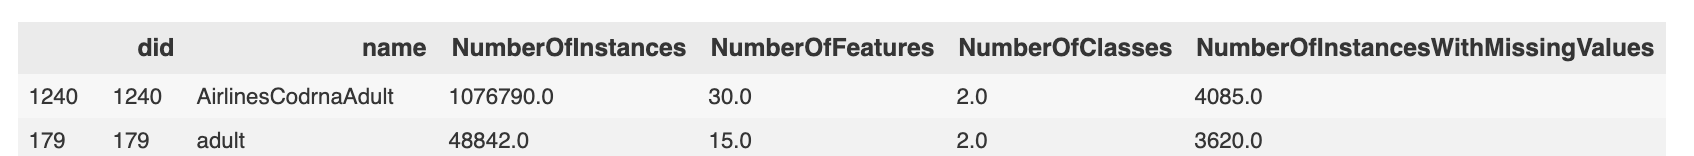
\includegraphics[width=1\textwidth]{openml_eda3.png} 
    \caption{Number of data points distribution}
    \label{fig:openml-eda3}
\end{figure}

Analyzing the number of instances in the subset of datasets used in this study, it can be seen that most of the datasets have a relatively small number of instances, but a portion of them have more than $300000$ data points, in hope to cover more data-heavy models (\ref{fig:openml-eda2}).

\begin{figure}[!h]
    \centering
    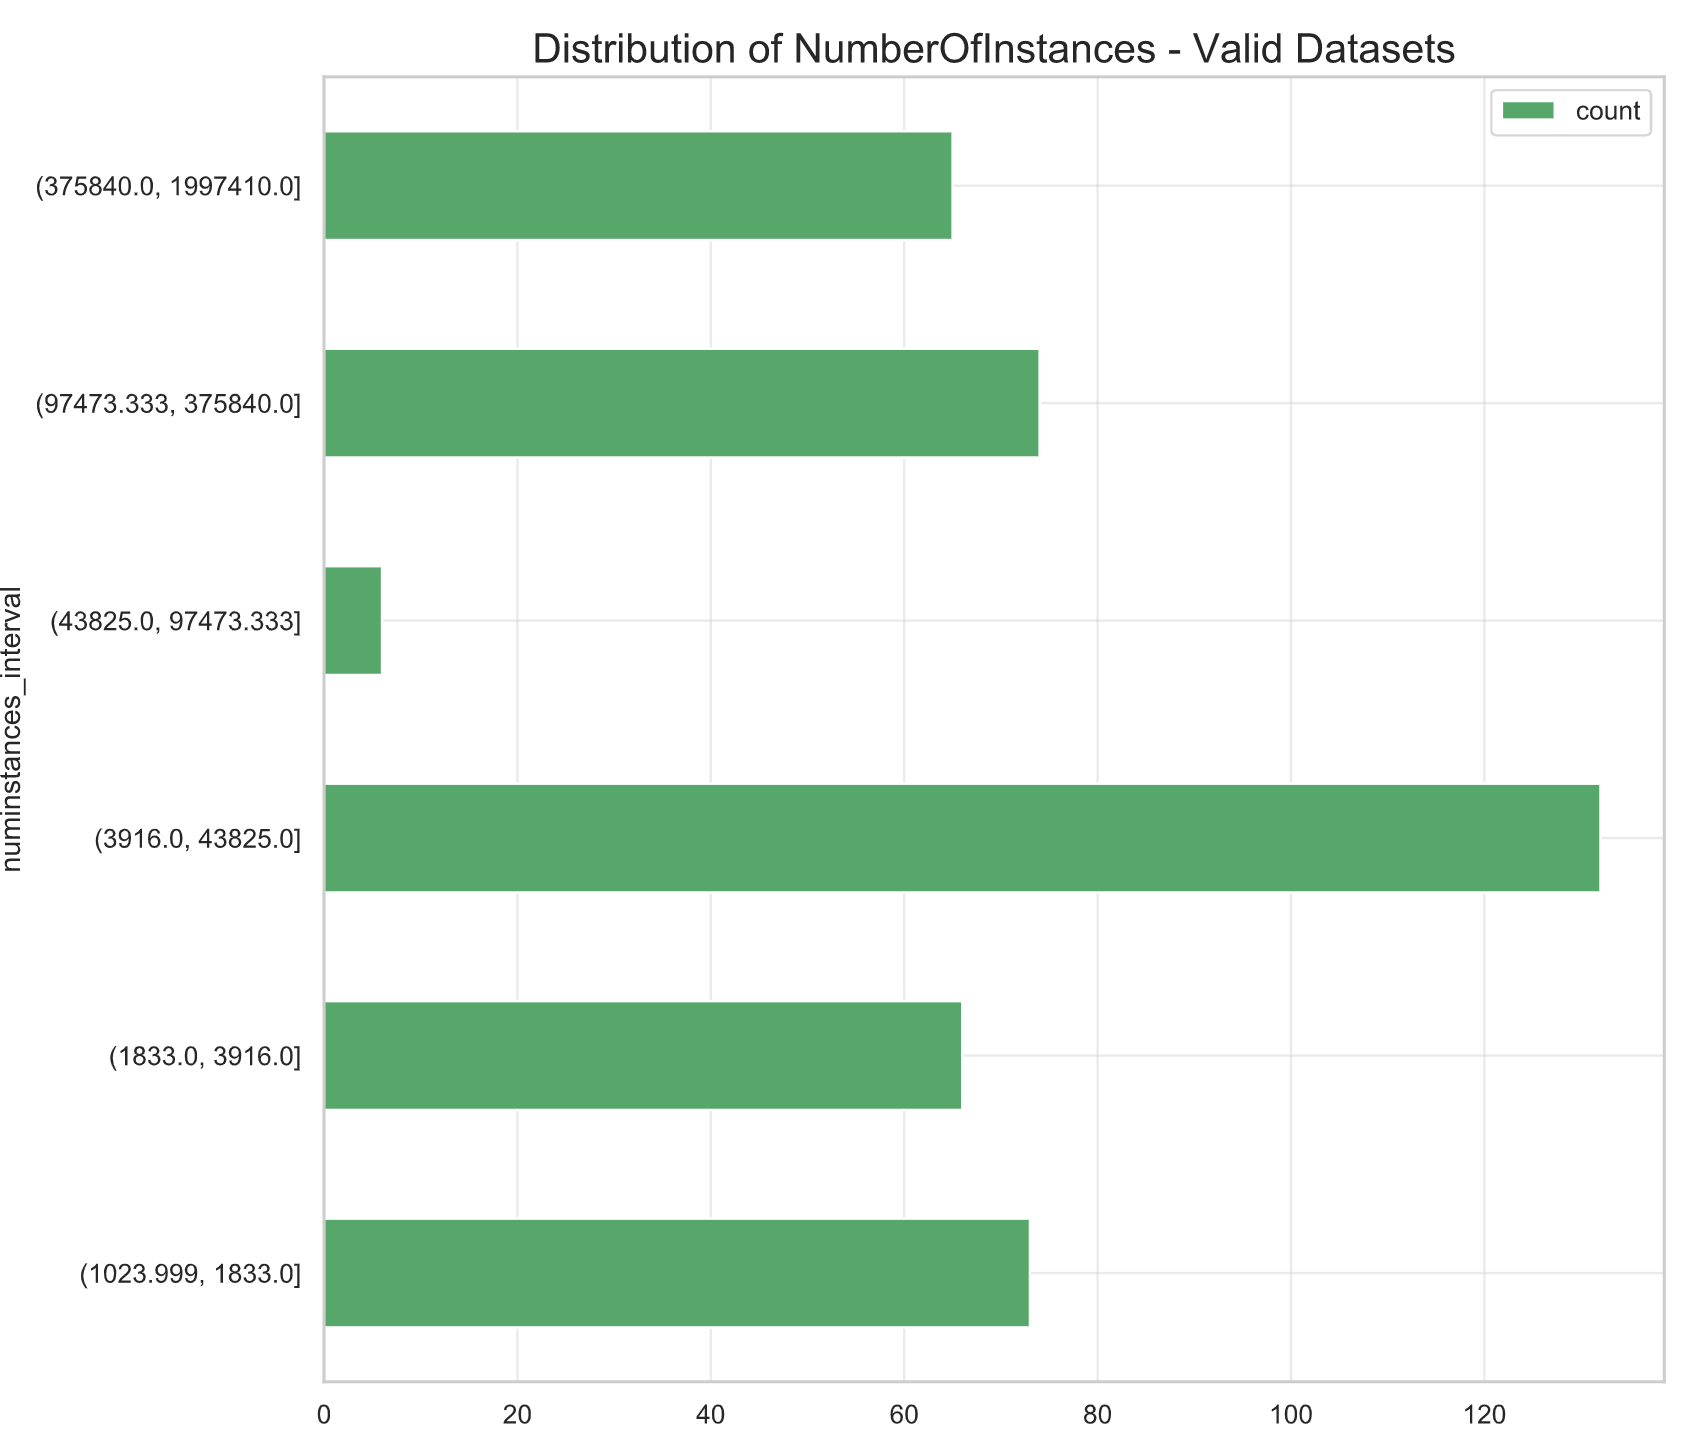
\includegraphics[width=.7\textwidth]{openml_eda2.png} 
    \caption{Number of data points distribution}
    \label{fig:openml-eda2}
\end{figure}

\newpage

\subsection{Data Cleaning}

In this study there are only two data cleaning steps, with the objective to keep the cleaned dataset as close as possible to the original to not interfere with the experiment results.
\begin{enumerate}
    \item The OpenML provides an attribute describing which of the features in the dataset are the categorical features; In the dataset building process, the type of each variable is identified (using \textit{pandas-profiling} package), and from each identified feature as "categorical", remove all that aren't explicitly declared by the OpenML attributes;
    \item The data in each OpenML dataset doesn't follow a specific pattern, e.g. some datasets represent the \textbf{target} variable as a string (\textit{'y'} and \textit{'n'}), some are represented in floating point, boolean, etc. In the experiment pipeline, the \textbf{target} is converted to an integer, if possible. If not, the \textbf{target} is encoded using a \textit{label encoder}.
\end{enumerate}

%% ------------------------------------------------------------------------- %%
\section{Descriptive dataset statistics}
\label{dataset-aggregated-statistics}

To analyze subgroups of datasets and categorize each one of them, multiple statistics related to the structure of the dataset is calculated before any machine learning model is trained. Before the training process, the granularity of these statistics are feature-wise, which are then further aggregated in the result analysis step.

\textbf{Categorical features} are known to cause a \textit{prediction shift} in traditional gradient boosting models, as demonstrated in \cite{prokhorenkova2018catboost}. This shift is identified as a special kind of target leakage, which can also be caused in a preprocessing step of categorical features when using target statistics (e.g. using the target/mean encoding technique)\footnote{To fix this kind of problem in a dataset with many categorical features a new boosting algorithm was developed by \cite{dorogush2018catboost} called \textbf{Catboost}.}. As noted in the mentioned paper, LightGBM converts categorical features to gradient statistics at each step of the boosting process (as explained in section \ref{lightgbm-explanation}), which result in some information loss. To categorize datasets with relation to categorical features, in this work the following statistics related to categorical variables are calculated:

\begin{itemize}
    \item \textbf{cardinality}, is the number of unique categorical values of a given feature;
    \item \textbf{variance}, is  a simple measure of variability of a specific categorical feature.
    Let $|top_{j}|$ be the number of occurrences of the most frequent category in feature $j$, i.e. the column $\xmat_{:, j}$. Then, this metric is defined as the inverse of the ratio of occurrences of the most frequent category:

    $$categorical\_variability=1 - \frac{|top_{j}|}{|\xmat_{:, j}|}$$

    As an example, if 90\% of the values of a given feature is the same, then the categorical variability of the said feature is $0.1$.
\end{itemize}

For \textbf{numeric features}, the main specific statistic calculated is the sample \textbf{skewness} of each feature. Skewness is a degree of distortion of a distribution, and in this study it's calculated using the unbiased adjusted Fisher–Pearson standardized moment coefficient from \textit{pandas}. The skewness is also trying to measure the variability of the numeric features, and is used in the clustering of each dataset as a feature.

The pipeline also calculates other useful statistics for each feature, like the percentiles, number of NaNs, infinite values, mean, median, etc. They're useful in the exploratory step, but are not used when clustering the datasets in the result analysis step.

%% ------------------------------------------------------------------------- %%
\section{Hyperparameter space}

In section \ref{gbm-hyperparams} it's explained the basic hyperparameter used in LightGBM's gradient boosting algorithm. In this section the \textit{hyperparameter space} of the study is explained, along with a simple overview of the hypothesis behind each distribution choice related to LightGBM default hyperparameters.